
\begin{figure}[h]
\centering
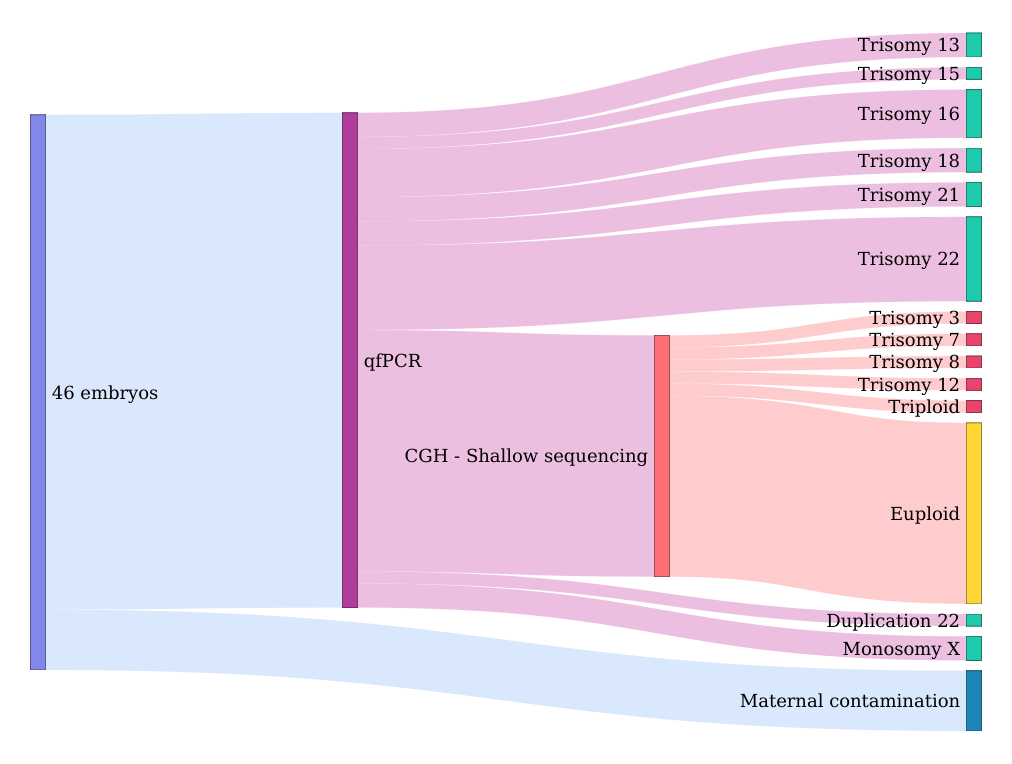
\includegraphics[width=0.7\textwidth]{fig/ibelieve.png}
\caption{\textbf{Outcome of the screening for aneuploidies in the embryos.} Screening on embryonic DNA by quantitative PCR, comparative hybridization and shallow sequencing finds aneuploidies in  56.6\% of the embryos, the most common being the trisomy of chromosome 22. In yellow the fraction of euploid embryos. }
\label{fig:presequencing}
\end{figure}

\begin{figure}[ht]
\centering
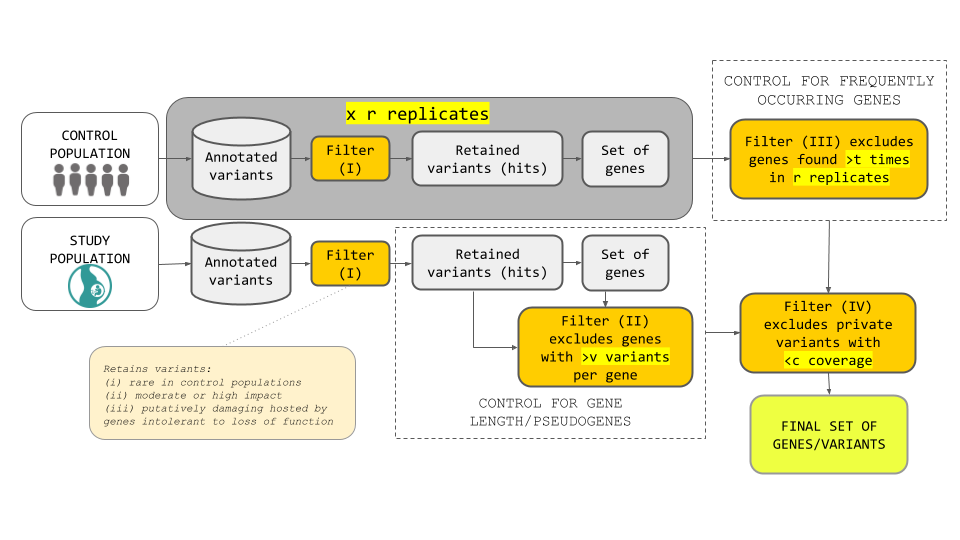
\includegraphics[width=\linewidth]{fig/pipeonly.png}
\caption{\textbf{Overview of the pipeline for prioritization of the genetic variants.} more text here } 
\label{fig:pipeline}
\end{figure}
%Genetic variants discovered in samples and controls are annotated and Filtered on the basis of the annotations (Filter I). In samples  Samples are first screened for the quality of DNA and maternal contamination and then analyzed for aneuploidies. \textbf{(B) Outcomes of the pipeline.} We estimate that 18\% of samples goes to sequencing....


\begin{figure}[ht]
\centering
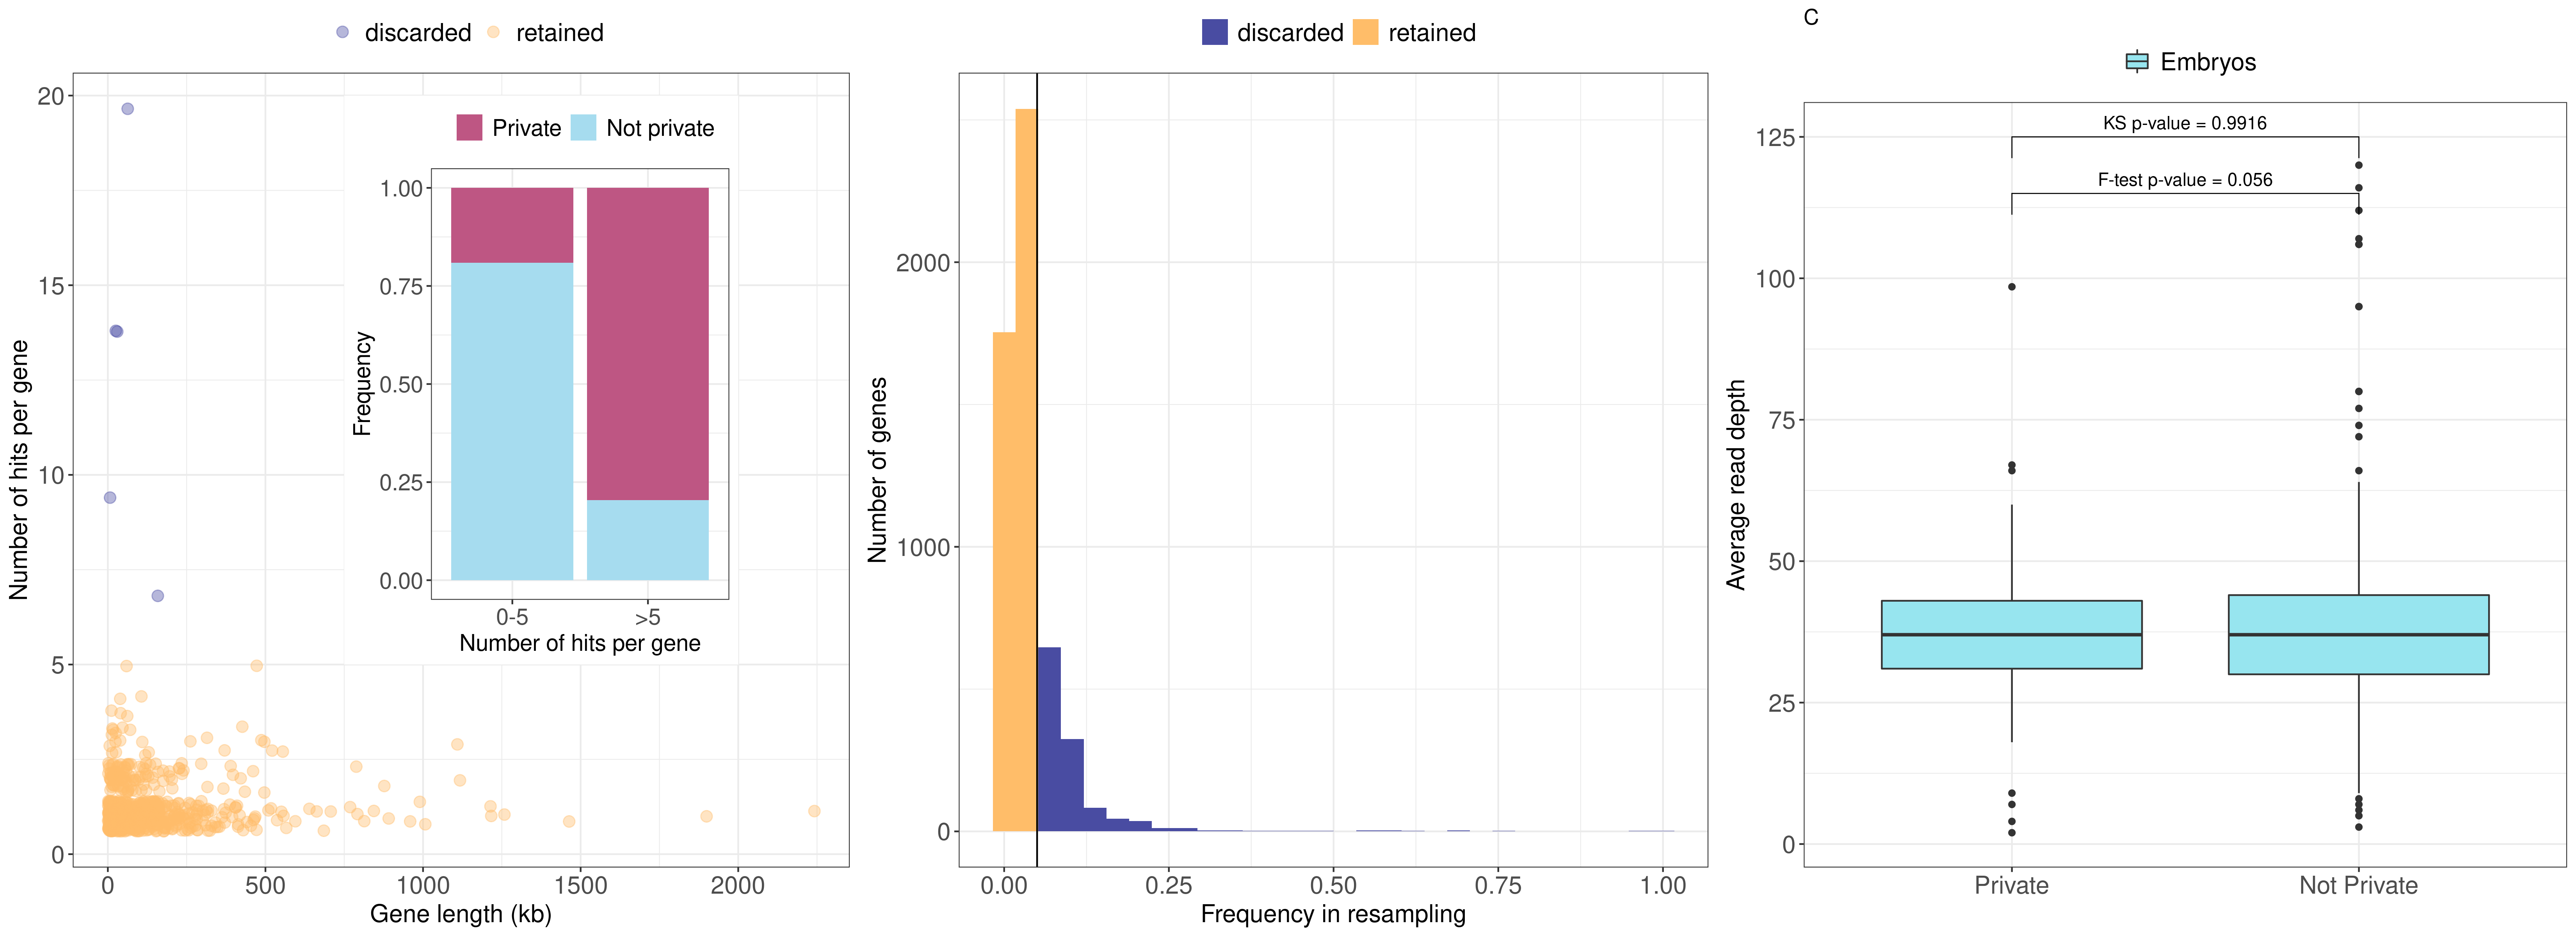
\includegraphics[width=\linewidth]{fig/filters_embryos.png}
\caption{\textbf{}}
\label{fig:filters}
\end{figure}

\begin{figure}[ht]
\centering
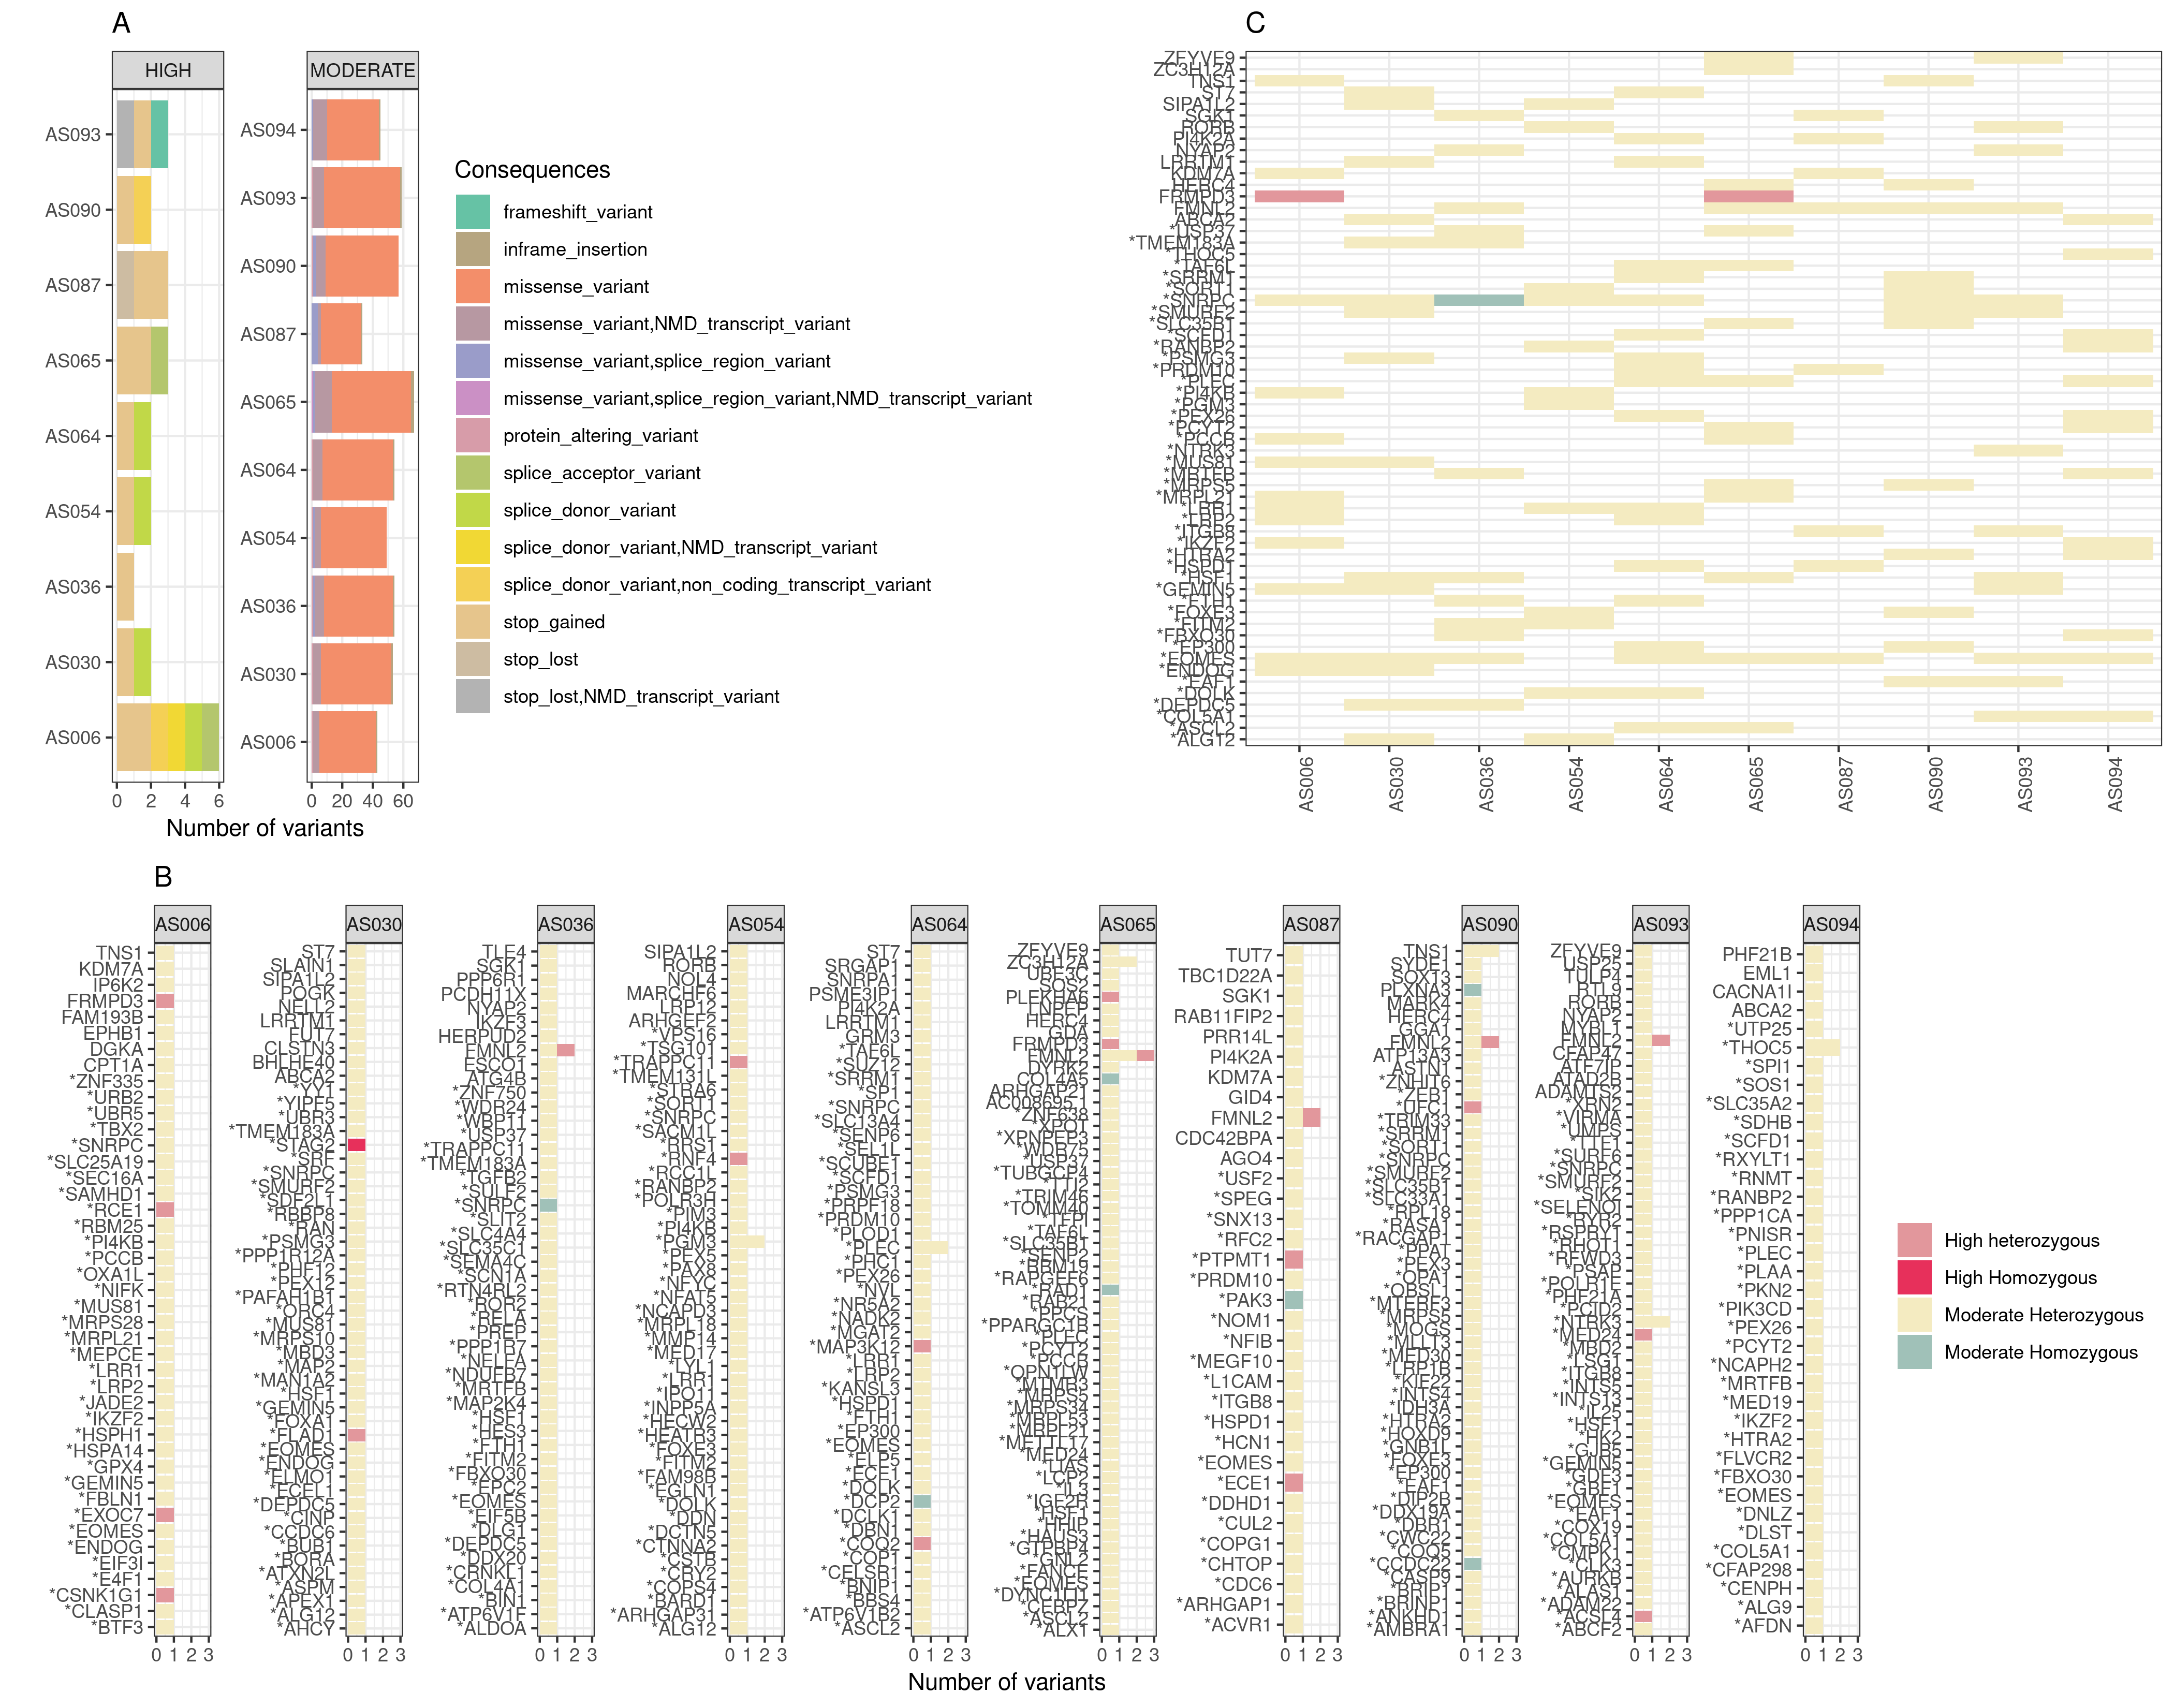
\includegraphics[width=\linewidth]{fig/panel_EmbryoResults.png}
%\caption{\textbf{} he occurrence of variants, their impact, and the count of the consequence allele per gene per embryo  }
\caption{\textbf{}}
\label{fig:resembryo}
\end{figure}

